\documentclass[11pt,a4paper]{article}
\usepackage[T1]{fontenc}
\usepackage[utf8]{inputenc}
\usepackage{mathpazo}
\usepackage[scaled=0.90]{helvet}
\usepackage{textcomp}
\usepackage{microtype}
\usepackage[margin=30mm,top=27mm,bottom=29mm]{geometry}
\usepackage{graphicx}
\usepackage{amsmath}
\usepackage{booktabs}
\usepackage{array}\newcolumntype{L}[1]{>{\raggedright\arraybackslash}p{#1}}
\usepackage[font=small,labelfont=bf,labelsep=period,skip=7pt]{caption}
\usepackage{fancyhdr}
\usepackage{titlesec}
\usepackage[hidelinks]{hyperref}
\usepackage{enumitem}
\usepackage[section]{placeins}
\setcounter{topnumber}{2}\setcounter{bottomnumber}{2}\setcounter{totalnumber}{3}
\renewcommand{\topfraction}{0.92}\renewcommand{\bottomfraction}{0.75}
\renewcommand{\textfraction}{0.08}\renewcommand{\floatpagefraction}{0.72}

\titleformat{\section}{\normalfont\large\bfseries}{\thesection.}{0.6em}{}
\titlespacing*{\section}{0pt}{16pt}{6pt}
\titleformat{\subsection}{\normalfont\normalsize\bfseries\itshape}{}{0em}{}
\titlespacing*{\subsection}{0pt}{10pt}{3pt}
\setlength{\parskip}{0pt}\setlength{\parindent}{1.4em}\linespread{1.05}

\pagestyle{fancy}\fancyhf{}
\renewcommand{\headrulewidth}{0.4pt}
\lhead{\footnotesize\itshape The Payoff Diagram Is Lying to You}
\rhead{\footnotesize Kittson}
\cfoot{\footnotesize\thepage}
\newcommand{\PnL}{P\&L}

\begin{document}

\begin{center}
{\LARGE\bfseries The Payoff Diagram Is Lying to You}\\[10pt]
{\large Simon Kittson}\\[14pt]
\end{center}

\begin{quote}\small\itshape
The hockey stick is the most widely deployed piece of risk communication in retail finance, and it describes one second of a position's life, under no probability measure at all. The expiry payoff diagram remains useful for explaining terminal contract geometry; it is incomplete as a display of mark-to-market risk because it suppresses time, volatility and a probability measure. This article sets out what the diagram cannot say, why the previous attempts to replace it did not stick, and a display standard that restores what it suppresses, together with the test that would settle whether it works.
\end{quote}

\vspace{6pt}
\noindent\fbox{\parbox{\dimexpr\linewidth-2\fboxsep-2\fboxrule\relax}{\small
\textbf{What this article contributes.} i) A formal separation of terminal payoff from mark-to-market \PnL{}. ii) A fixed small-multiple display indexed by elapsed time and implied-vol regime. iii) A conditional spot distribution per cell with spot--vol correlation, implied and realised vol distinguished, calibrated to Apple. iv) Cell-level $P(\Pi>0)$, $E[\Pi]$ and a 5\% loss quantile. v) A frequency-framed alternative and an expert/retail mode split. vi) A powered user study against the payoff diagram and current broker tools.}}
\vspace{6pt}

\section{The most successful wrong chart in finance}

\noindent Every options platform, textbook and broker education page leads with the same picture: profit or loss against terminal share price, and a kinked line. By volume of daily impressions it is surely the most successful piece of financial data visualisation ever produced, and retail education still teaches it as \emph{the} risk visual whilst conceding that most positions are closed before expiration.

The diagram is very good at what it is for: comparing structures at expiry, locating break-evens and maximum loss, teaching the shape of optionality. The charge is that a terminal-payoff display has been institutionalised as a \emph{risk} display, and as a risk display it fails, which is not new. Israelov and Nielsen (2014) listed among their eight myths of covered-call investing the belief that ``risk exposure can be expressed in a payoff diagram'', and Wystup (2019), in these pages, put the confusion of payoff diagrams with \PnL{} diagrams first among his common misconceptions. It answers one question, what the position is worth at expiry; what it is worth \emph{now}, what happens if implied volatility moves, and how \emph{likely} any outcome is lie outside its vocabulary.

Two structural omissions do the damage.

\textbf{It shows one instant of a path-dependent experience.} Let $u$ be the time elapsed since the trade was put on and $\tau = T - u$ the time remaining. Write the mark-to-market \PnL{} per share of a European option position as
\[
\Pi(S,u;\sigma) \;=\; V(S,\tau;\sigma) - V(S_0,T;\sigma_0), \qquad \tau = T-u,
\]
where $V(S,\tau;\sigma)$ is the Black--Scholes value with $\tau$ to run, $\sigma$ the implied volatility at the unwind, and the second term the premium paid. The payoff diagram is the single slice at $u = T$, at which point, conveniently, $\sigma$ has vanished from the problem. For every $u < T$ the position the investor actually holds, and the price at which they can exit, is a smooth curve in $S$ that may sit far from the terminal kink (Figure~1).

\begin{figure}[htbp]
\centering
\setcounter{figure}{0}
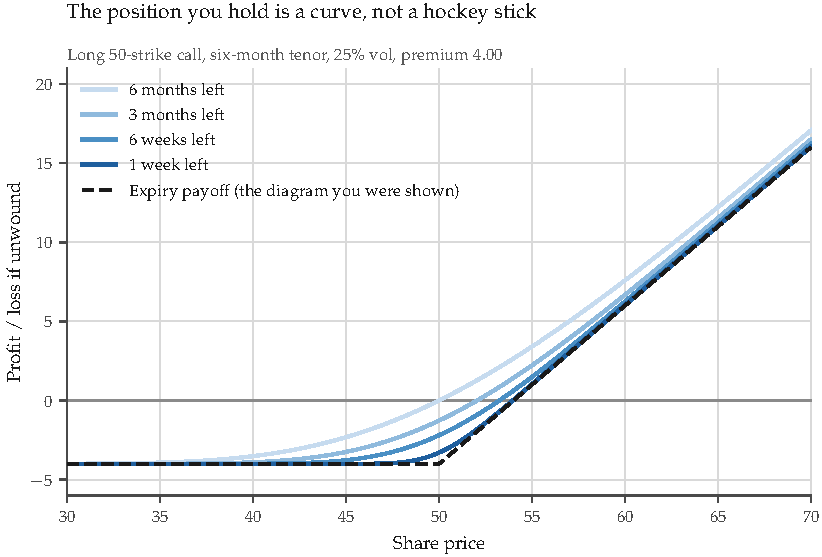
\includegraphics[width=\linewidth]{v2_fig1.pdf}
\caption{Long 50-strike call (six months, $\sigma = 25\%$, $r = 4\%$): expiry payoff versus mark-to-market value per share at 6 months, 3 months, 6 weeks and 1 week remaining ($\tau$). \emph{Status: scenario at constant implied vol, not a forecast.}}
\end{figure}

\textbf{It carries no measure.} The horizontal axis extends impartially in both directions, as though every terminal price were equally worth contemplating; the geometry of the payoff is presented whilst the distribution it will be integrated against is suppressed. A risk display without a measure is not a simplification; it is half a pricing kernel masquerading as the whole.

Neither omission mattered when the audience was structurers who carried the missing surfaces in their heads. In the second quarter of 2026 zero-days-to-expiry contracts accounted for roughly 65\% of SPX options volume by Cboe's own reporting (Cboe, 2026a), with retail flow among the principal drivers, and at 0DTE tenors the intraday path and the vol dynamics \emph{are} the trade. The consequences are measured, and Brown (2022) asked in these pages whether individual investors should trade options at all: they underperform (Bauer, Cosemans and Eichholtz, 2009), the modern flow is short-dated and near the money (Bogousslavsky and Muravyev, 2024), and de Silva, Smith and So (2026) show retail traders buying options ahead of earnings in anticipation of volatility that is already in the price, and losing systematically when it collapses. That is a population-level loss in exactly the dimension the payoff diagram hides. Eaton, Green, Roseman and Wu (2026) add the twist: retail flow now measurably distorts the implied volatility surface itself. A cohort large enough to move the parameter is shown, at the point of sale, a picture in which it does not exist.

\section{What the diagram cannot show you: a worked irritant}

\noindent Consider a six-month long straddle: $S_0 = K = 50$, $r = 4\%$, $\sigma_0 = 25\%$, no dividends; premium $7.02$ (call $4.00$, put $3.01$), break-evens near 43 and 57. Three weeks in, let implied volatility reprice from 25\% to 45\% with spot roughly unchanged. \textbf{Figure~2} shows $\Pi(S, u = 21/250)$ under three regimes. Under the spiked regime the \emph{entire} curve sits above zero: the minimum over all spot values is $+4.21$ on the $7.02$ premium, and there is no share price at which the unwind loses. Table~1 decomposes the gain at unchanged spot: theta cost $0.61$, twenty vol points at a vega of $0.25$ contributed $5.06$, and there is no second-order term because an at-the-money straddle's vega is almost linear in $\sigma$. The $+4.44$ at $S = 50$ and the $+4.21$ floor near $S = 47.2$ are different numbers; the floor is what the display should print.

\begin{figure}[htbp]
\centering
\setcounter{figure}{1}
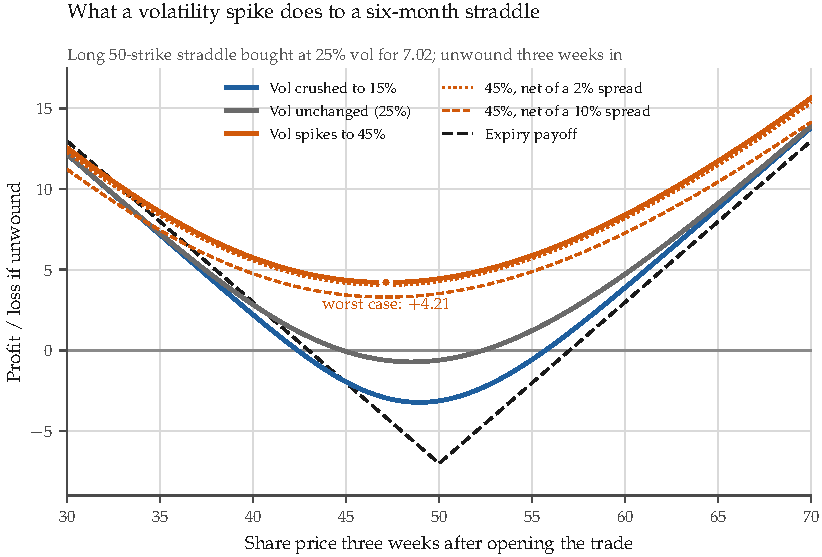
\includegraphics[width=\linewidth]{v2_fig2.pdf}
\caption{Long 50-strike straddle bought at $\sigma_0 = 25\%$ for 7.02: unwind \PnL{} per share at $u = 21/250$ under $\sigma_I \in \{15\%, 25\%, 45\%\}$, with expiry payoff dashed. Minimum \PnL{} under the 45\% regime is $+4.21$ near spot 47, and the minimum is global. The two thinner orange curves net a 2\% and a 10\% proportional bid--ask spread from the 45\% case; the floor survives both. \emph{Status: scenario (flat repricings), not a forecast; mid-market except where stated.}}
\end{figure}

\begin{table}[htbp]
\centering\small
\caption{Unwind \PnL{} at unchanged spot, three weeks into the six-month straddle, decomposed.}
\begin{tabular}{@{}lr@{}}
\toprule
Component & \PnL{} \\
\midrule
Theta: three weeks of decay at $\sigma = 25\%$ & $-0.61$ \\
Vega: $0.253$ per vol point $\times$ 20 points & $+5.06$ \\
Convexity in $\sigma$ (residual) & $\phantom{+}0.00$ \\
\midrule
Total at $S = 50$, before frictions & $+4.44$ \\
\bottomrule
\end{tabular}
\end{table}

The mirror image is the post-earnings ritual, $\sigma$ crushed to 15\% and the position losing at spot levels the diagram marks as safe; de Silva, Smith and So (2026) make that a measured phenomenon: the trader bought a volatility the display never showed and the event then removed.

Frictions deserve numbers. The curves are mid-market; an unwind crosses the bid--ask twice on each leg. Table~2 prices the round trip under stated spread assumptions: a 2\% spread costs 4\% of the floor, a mid-cap name at 10\% a fifth of it, and a retail-sized multi-leg order meeting a spread of the order of 20\% loses nearly half the windfall. Figure~2 draws the 2\% and 10\% cases and the floor survives both, at $+4.0$ and $+3.3$. The smile is likewise suppressed: a flat 45\% repricing is a scenario, not a calibration. Both effects bias the pictures optimistic, and both are also invisible on the standard diagram. None of this is news to anyone who marks a book; the point is that the \emph{display} at the point of sale cannot say it. The Greeks say it; however, the Greeks are local derivatives, and what the holder needs is the finite-displacement picture, which is what a chart is for.

\begin{table}[htbp]
\centering\small
\caption{Round-trip friction on the Figure~2 unwind under stated bid--ask spread assumptions (spread as a fraction of mid, half crossed on entry at 7.02 and half on exit at 11.46).}
\begin{tabular}{@{}lrrr@{}}
\toprule
Spread assumption & Round trip & Share of the 4.21 floor & Net \PnL{} at unchanged spot \\
\midrule
2\% (liquid index or large cap) & 0.18 & 4\% & $+4.26$ \\
5\% & 0.46 & 11\% & $+3.98$ \\
10\% (mid-cap single name) & 0.92 & 22\% & $+3.52$ \\
20\% (illiquid, retail multi-leg) & 1.85 & 44\% & $+2.60$ \\
\bottomrule
\end{tabular}
\end{table}

\section{Why the previous answers did not stick}

\noindent The problem has been attacked three times, and the three failures share a diagnosis.

\subsection{The third dimension}

Gresh, Rogowitz, Tignor and Mayland (1999) rendered option value over the tenor as interactive 3D surfaces; Fei and Prakash (2001) gave profit bands their own planes in a volume rendering. Both reached for depth to hold spot, time and volatility. Munzner (2014) ranks depth among the weakest visual channels, for occlusion, ambiguity and the cost of rotating to compare; her rule, \emph{no unjustified 3D}, was written for this case, Ko et al.\ (2016) record the same complaints from finance, and no mainstream package renders payoff surfaces in 3D today. The planar alternative is old and better: \textbf{small multiples} (Tufte, 1983), a grid of miniature charts on common scales, indexed by the variables one would otherwise have encoded in depth.

\subsection{The uncertainty literature}

Small multiples solve time and volatility, not the measure, and the recent literature is uncomfortable reading for anyone proposing shaded bands. Correll and Gleicher (2014) showed that error bars are misread even by trained audiences; Hullman, Resnick and Adar (2015) that animated hypothetical outcome plots outperform static intervals; Fernandes, Walls, Munson, Hullman and Kay (2018), with transit riders in the field, that quantile dotplots beat shaded intervals, most of all for the least expert. Joslyn and Savelli (2021) name the failure, the \emph{deterministic construal error}, in which a non-expert reads the edge of a band as a boundary and its interior as a certainty, and Padilla, Kay and Hullman (2022) conclude that frequency framing is the robust choice for non-experts. Section~4 therefore offers both encodings and says which is for whom.

\subsection{The brokers}

Table~3 records what exists as at September 2026. Interactive Brokers' Option Analytics bends a value curve by ``changing volatility assumptions, stepping closer to expiration and adjusting the price of the underlying'': omission one repaired, one scenario at a time. Its web order ticket, seen on 4 September 2026 for a zero-day Apple call, is the point of sale itself: a ``performance profile'' of maximum loss, break-even and maximum return, a P\&L line against price at a selectable date, a spot-shock ladder from $-30\%$ to $+10\%$ with the Greeks at each step, no volatility control, and beneath it a ``market implied probability of profit'' of 9.5\%, at expiry. Its Probability Lab reports a ``percentage likelihood of profit'' against a market-implied distribution: omission two repaired, but only ``at the time the option expires''. thinkorswim quotes a probability of expiring and an expected move, draws a probability-of-expiring cone on its price charts, and bends its risk profile under slider control; Power E*TRADE's Snapshot Analysis prints a probability of profit against an expiry-only risk graph. Beneath the brokers, OptionStrat and OptionsProfitCalculator.com lay out ``the expected profit and loss of your trade at various prices and dates'' on one fixed table, with an implied-vol slider and a probability of profit ``on the day of expiry''. The calculators have already fixed the time axis; what they have not fixed is what the rest of this article is about.

\begin{table}[htbp]
\centering\small
\caption{Where the two omissions are repaired in mainstream retail tooling, from the vendors' own documentation as at 4 September 2026 (Interactive Brokers, 2026a,b; Charles Schwab, 2026; E*TRADE, 2026; OptionStrat, 2026; OptionsProfitCalculator, 2026), and, for the IBKR Client Portal ticket, from direct inspection in a paper-trading account on the same date. The calculators have fixed the time axis; no surface draws a measure on the intermediate-date picture, and none shows volatility regimes side by side.}
\begin{tabular}{@{}L{3.4cm}L{3.0cm}L{3.0cm}L{4.1cm}@{}}
\toprule
Tool & Intermediate dates? & Measure on the \PnL{} view? & Scenarios shown together? \\
\midrule
Static payoff diagram & No & No & No \\
IBKR Option Analytics (TWS) & Yes, by slider & No & One at a time \\
IBKR Client Portal ticket (seen) & Yes, by date selector & No; expiry-only number & One date; spot ladder, no vol axis \\
IBKR Probability Lab & Expiry only & Yes, at expiry & One distribution \\
thinkorswim Risk Profile & Yes, by slider & Separate readouts; cone on the price chart & One at a time \\
Power E*TRADE Snapshot Analysis & Expiry only & Expiry-only number & One at a time \\
OptionStrat & Yes, fixed date table & Expiry-only number & Dates together; vol by slider \\
OptionsProfitCalculator & Yes, fixed date table & Expiry-only number & Dates together; vol fixed \\
Proposed grid (Section 4) & Yes, fixed rows & Yes, per cell & Twelve at once \\
\bottomrule
\end{tabular}
\end{table}

Two things stop short, and they are the two omissions in modern dress. Volatility is everywhere a \emph{slider}: the user drags a control and compares the current view with their memory of the previous one, the 3D-rotation problem reincarnated with better manners. Small multiples exist so that the eye does the differencing rather than the hippocampus. And no surface commits to a measure on the \PnL{} view at an intermediate date; where probability exists it lives at expiry or in a separate readout, and nowhere is it conditioned on the volatility regime the user is looking at. The distinction pressed here is not ``richer analytics'' but a \emph{display standard} that begins where the calculators stop: volatility as a facet rather than a slider, and a measure, conditional on that facet, drawn on every cell.

\section{The proposal}

\noindent For a position with tenor $T$:

\begin{itemize}[leftmargin=1.4em,itemsep=3pt,topsep=6pt]
\item \textbf{Rows:} elapsed times $u \in \{\tfrac14 T, \tfrac12 T, \tfrac34 T, T\}$, each priced with $\tau = T - u$ to run.
\item \textbf{Columns:} three implied-volatility regimes $\{\sigma_{\text{low}}, \sigma_0, \sigma_{\text{high}}\}$, user-set, each a representative point for a bucket (below 20\%, 20\% to 35\%, above 35\% in the base case). The columns are scenarios, not forecasts; the probability printed in a cell is the model-implied probability of the bucket.
\item \textbf{Each cell:} the unwind curve $\Pi(S,u;\sigma_I)$ per share on common axes, mid-market unless a spread is supplied.
\item \textbf{Two volatilities, not one.} The band's width is set by the \emph{realised} volatility $\sigma_R$ over $[0,u]$, a different object from the implied vol that prices the curve. The default $\sigma_R = \sigma_I$ is stated on the face of the picture, because a silently overloaded parameter is the sin the display exists to correct.
\item \textbf{The measure, restored twice.} Within a cell, the 68\% and 95\% bands of $S_u$ \emph{conditional on the regime}; across cells, each regime's probability, so that three columns are never weighted equally when the market does not. Both follow from one small joint model, an assumption rather than a derivation: $\ln\sigma_u$ normal with vol-of-vol $\nu$, $\ln S_u$ lognormal and correlated with it at $\rho$. Conditional on the regime the band's centre shifts by $\rho\,\sigma_R\sqrt{u}\,z$, $z$ being the standardised vol move, and its variance shrinks to $(1-\rho^2)\sigma_R^2 u$; $\rho = 0$ recovers the independent grid (Appendix~A).
\item \textbf{The question answered.} Each cell prints $P(\Pi > 0)$, $E[\Pi]$ and the 5\% loss quantile $Q_{5\%}(\Pi)$, so the reader is not asked to integrate a curve against a band by eye, the one operation the structurer can do in their head and the retail user cannot. Probability of profit and expected \PnL{} summarise the centre of the distribution; risk lives in its left tail and in what the model omits: loss quantiles and expected shortfall, maximum loss, drawdown, the margin call, model and liquidity risk. The grid carries the first on its face and shows the rest as geometry; it does not claim that two centre statistics are a risk measure.
\end{itemize}

Figure~3 corrects the intuition the bands rest on: a 50 share at a sedate 20\% volatility spans roughly 38 to 67 at 95\% six months out, and the straddle's upper break-even sits inside that range within six weeks.

\begin{figure}[htbp]
\centering
\setcounter{figure}{2}
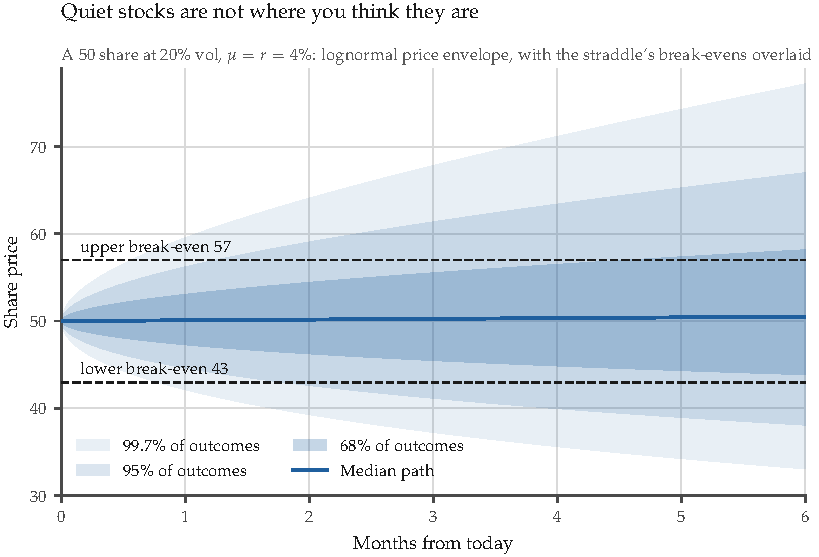
\includegraphics[width=\linewidth]{v2_fig3.pdf}
\caption{Lognormal price envelope (68/95/99.7\%) for a 50 share at $\sigma = 20\%$, $\mu = r = 4\%$, over six months, with the straddle's break-evens (43/57, priced at 25\%) overlaid. \emph{Status: model-implied under a lognormal spot process with a stated volatility; risk-neutral drift.}}
\end{figure}

\begin{figure}[p]
\centering
\setcounter{figure}{3}
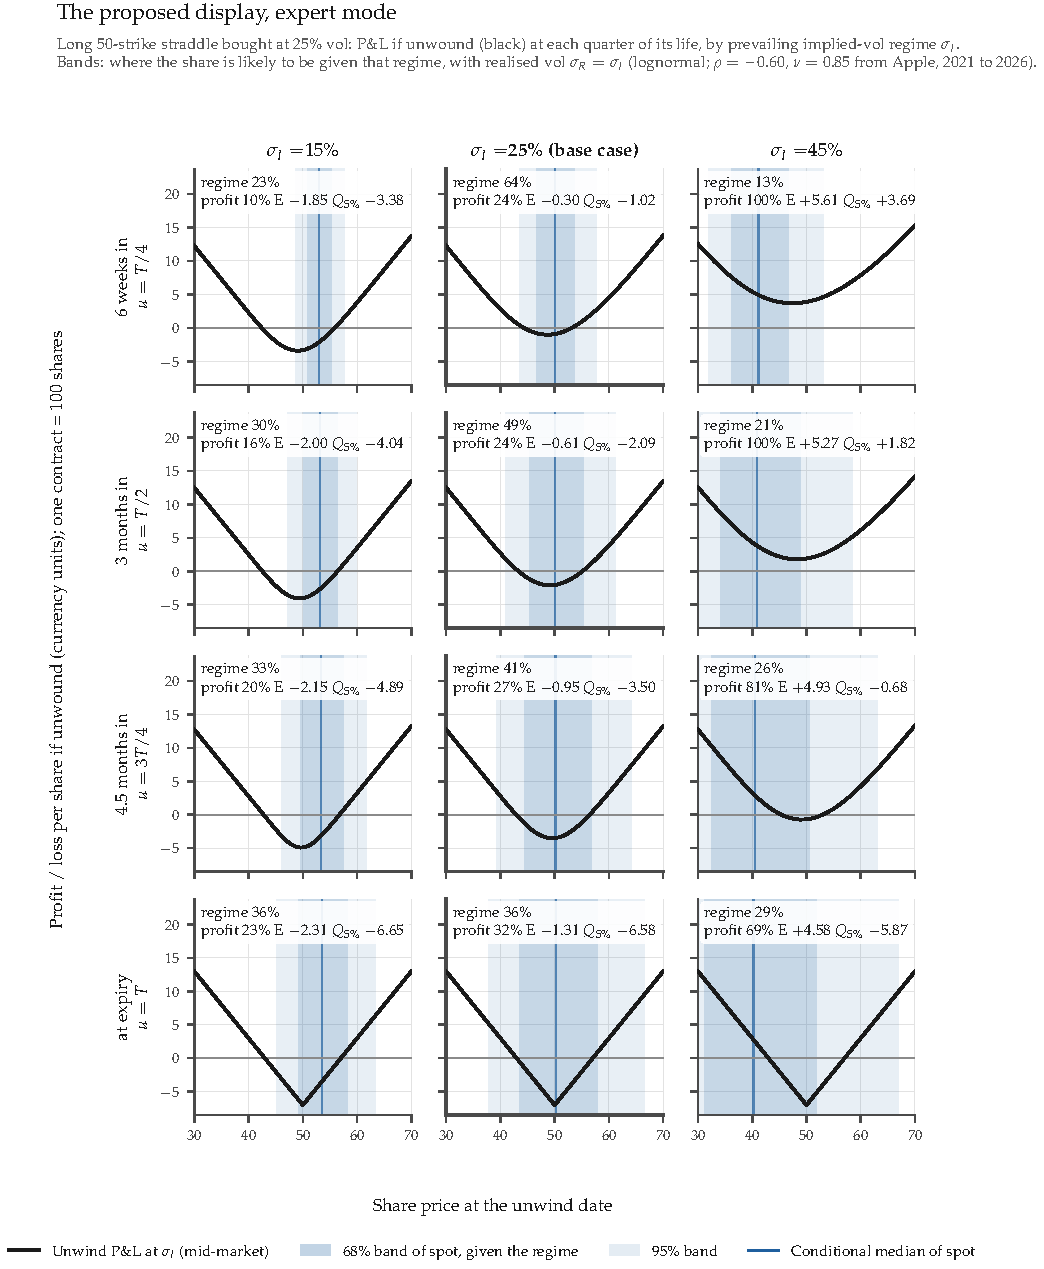
\includegraphics[width=\linewidth]{v2_fig4.pdf}
\caption{The proposed display, expert mode: unwind \PnL{} per share for the straddle at each quarter of its life (rows, elapsed time $u$) by implied-vol regime $\sigma_I$ (columns; base case in bold). Bands: 68\% and 95\% of spot at that date \emph{conditional on the regime}, with $\sigma_R = \sigma_I$; the thin line is the conditional median. Each cell prints the model-implied probability of its regime bucket, the probability of unwinding at a profit, the expected \PnL{} and the 5\% loss quantile. Mid-market throughout. \emph{Status: curves are scenarios; bands and statistics are model-implied under Appendix~A with $\rho$ and $\nu$ estimated from Apple, 2021 to 2026.} Bottom row: identical curves, different measures.}
\end{figure}

\textbf{Figure~4} shows the result under $\rho = -0.6$ and $\nu = 0.85$, which are not invented: they are Apple's spot--vol correlation and vol-of-vol over the five years to September 2026, estimated from Cboe's VXAPL index against Apple's closes (Appendix~A). Apple's implied vol on the day of writing was 25.8\%, by coincidence the base case. The grid reads like a comic strip. Down a column is theta made visible, sagging gently through the first half of the tenor and viciously in the last quarter; across a row is vega as a scenario rather than a partial derivative. The bottom row carries the thesis: at expiry the three curves are identical, the V is the V, whilst the bands differ, and the numbers say by how much: the same terminal payoff is unwound at a profit 23\% of the time in the low-vol column, 32\% in the middle and 69\% in the high. Volatility has stopped affecting the payoff function and has spent six months determining \emph{which part of it you would land on}; no single-panel display can make that statement.

Two features answer objections the independent grid could not. The 45\% column's band is centred near 41, not 50: a name whose implied has reached 45\% has usually fallen to get there, and Apple's six-month windows ending above 35\% vol show a fall of about 19\% relative to the middle bucket (Appendix~A). And the regime probabilities are printed: at six weeks the high-vol column is a 13\% event and the low-vol column a 23\% one. The grid as first built committed at its columns the sin it accused the diagram of at its axis; the repair is two parameters and one line of algebra.

\subsection{Two modes}

Section~3 flagged that shaded bands are the encoding the uncertainty literature predicts to underperform for this audience; the resolution is two modes of one specification. \emph{Expert mode} is Figure~4: continuous bands that compose with the curve and numerical summaries in every cell, for the reader who already carries the surface in their head. \emph{Retail mode} replaces bands with frequency-framed dots and counts; it is the point-of-sale display and the one Section~7 tests. \textbf{Figure~5} shows the three-months-in row in retail mode: twenty dots, each an equally likely share price under the cell's measure, coloured by whether the position unwinds at a profit there. The probability of profit is a count, 3 of 20, 4 of 20, 20 of 20, and the deterministic construal error has no edge to attach to. Nothing in the specification changes if the dots win, as the literature predicts they will.

\begin{figure}[htbp]
\centering
\setcounter{figure}{4}
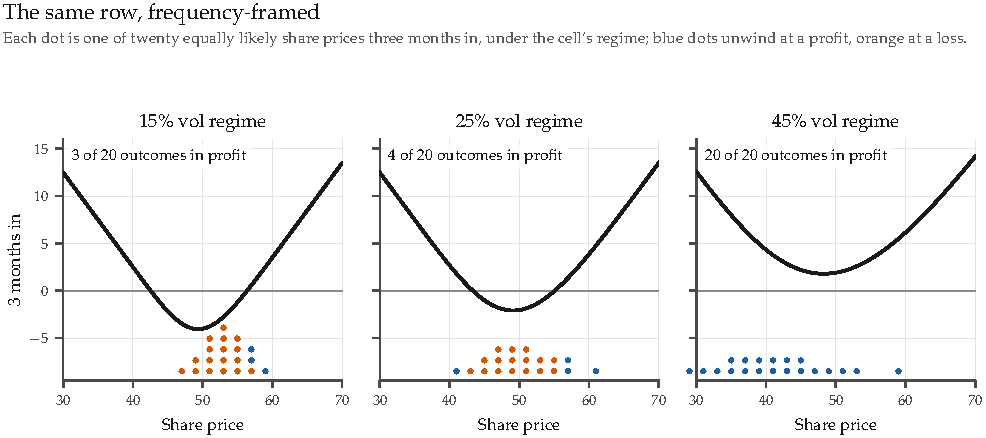
\includegraphics[width=\linewidth]{v2_fig5.pdf}
\caption{Retail mode: the three-months-in row of Figure~4 with the band replaced by a twenty-dot quantile dotplot of spot under each cell's conditional measure. Blue dots unwind at a profit, orange at a loss. \emph{Status: model-implied, same model and parameters as Figure~4.}}
\end{figure}

\subsection{Three other positions}

The display is not a case for buying options, and Figure~6 is there to prove it: the three-months-in row for a long call, a short 45/40 put spread and a short 50-strike straddle, on the same underlying and the same measure. For the long call the grid adds what Figure~1 added. For the put spread it adds what a credit seller most needs and the terminal diagram least shows: how much of the likely range lies beyond the short strike, and that in the high-vol column the 5\% loss quantile, $-3.78$, sits within $0.4$ of the maximum loss of $4.14$. For the short straddle it is the mirror of Figure~4, and a harder picture: in the 45\% column the probability of an unwind at a profit is nil, the expected loss is $-5.27$ on a $7.02$ credit, and the 5\% quantile is $-12.32$, a loss the payoff diagram shows as a plateau and the margin department shows as a phone call. The grid is neutral; the trades it treats most harshly are simply the ones whose terminal diagrams look safest.

\begin{figure}[htbp]
\centering
\setcounter{figure}{5}
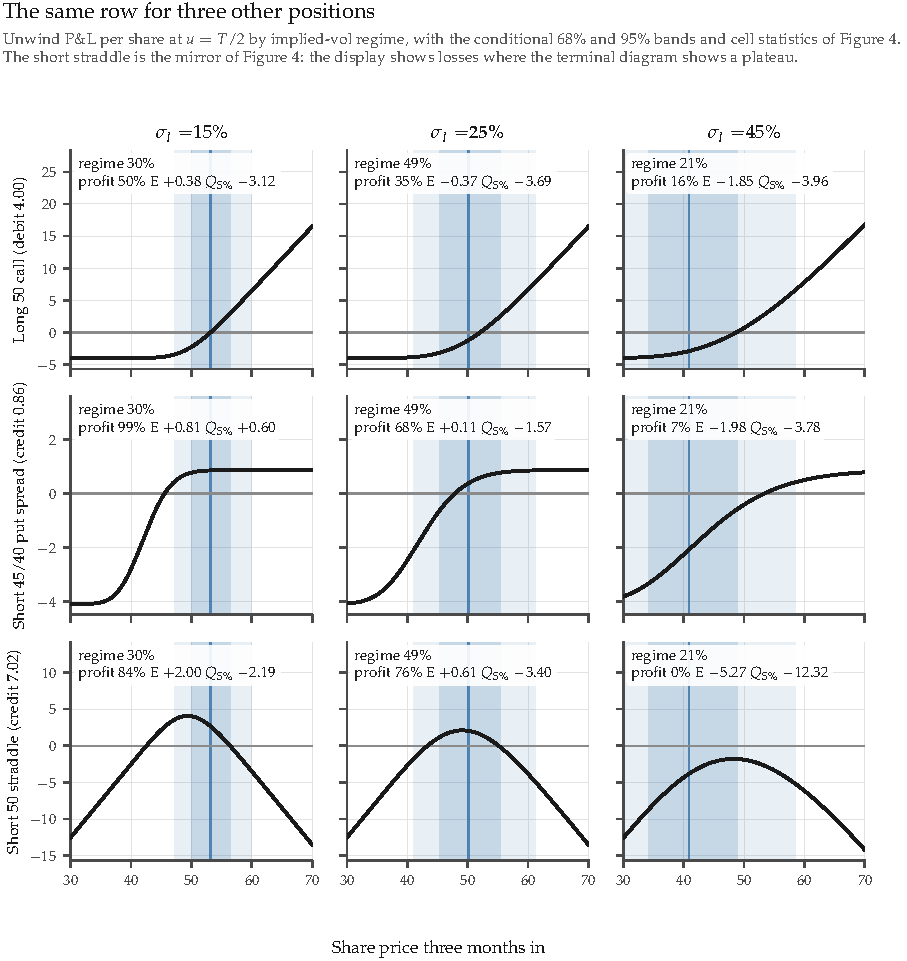
\includegraphics[width=\linewidth]{v2_fig7.pdf}
\caption{Robustness: the three-months-in row for a long 50-strike call, a short 45/40 put spread (credit 0.86) and a short 50-strike straddle (credit 7.02), same underlying, measure and cell statistics as Figure~4. \emph{Status: model-implied; same model and parameters as Figure~4.}}
\end{figure}

\subsection{Zero days to expiry: what survives and what does not}

\textbf{Figure~7} rebuilds the grid for an at-the-money straddle on an index at 100, bought at the open at 18\% for $0.905$ points, rows at one, three and five hours and the close, columns at 12\%, 18\% and 30\%. The joint model does not transfer: intraday vol moves are jumps, and a lognormal vol-of-vol prices a 12-to-30 move within three hours as a ten-sigma event, which it is not, so the grid is drawn with $\rho = 0$, without regime probabilities, and says so. What survives is instructive. The bands collapse to half a percent of spot at one hour and two percent by the close, so the picture is gamma against theta inside a two-point window. Expected \PnL{} is constant down each column, $-0.30$, $0.00$, $+0.60$, because without drift or correlation the expected unwind value does not depend on when it happens; the probability of profit does, rising through the day in the low- and base-vol columns (1\% to 23\%, 32\% to 42\%) and falling in the high-vol column (100\% to 63\%) as the vega cushion decays. The grid answers a question the hockey stick cannot pose: \emph{when} the trade is best unwound in each regime. What does not survive, and would need a jump-based regime model rather than a diffusion: i) jumps and event-time clustering in spot and vol; ii) intraday seasonality, with realised variance concentrated at the open and close whilst the implied number is an annualised average; iii) execution latency and a spread that is a large fraction of a sub-point premium; iv) settlement on the final print rather than the last trade. Halts and early exercise do not arise for cash-settled European index options.

\begin{figure}[p]
\centering
\setcounter{figure}{6}
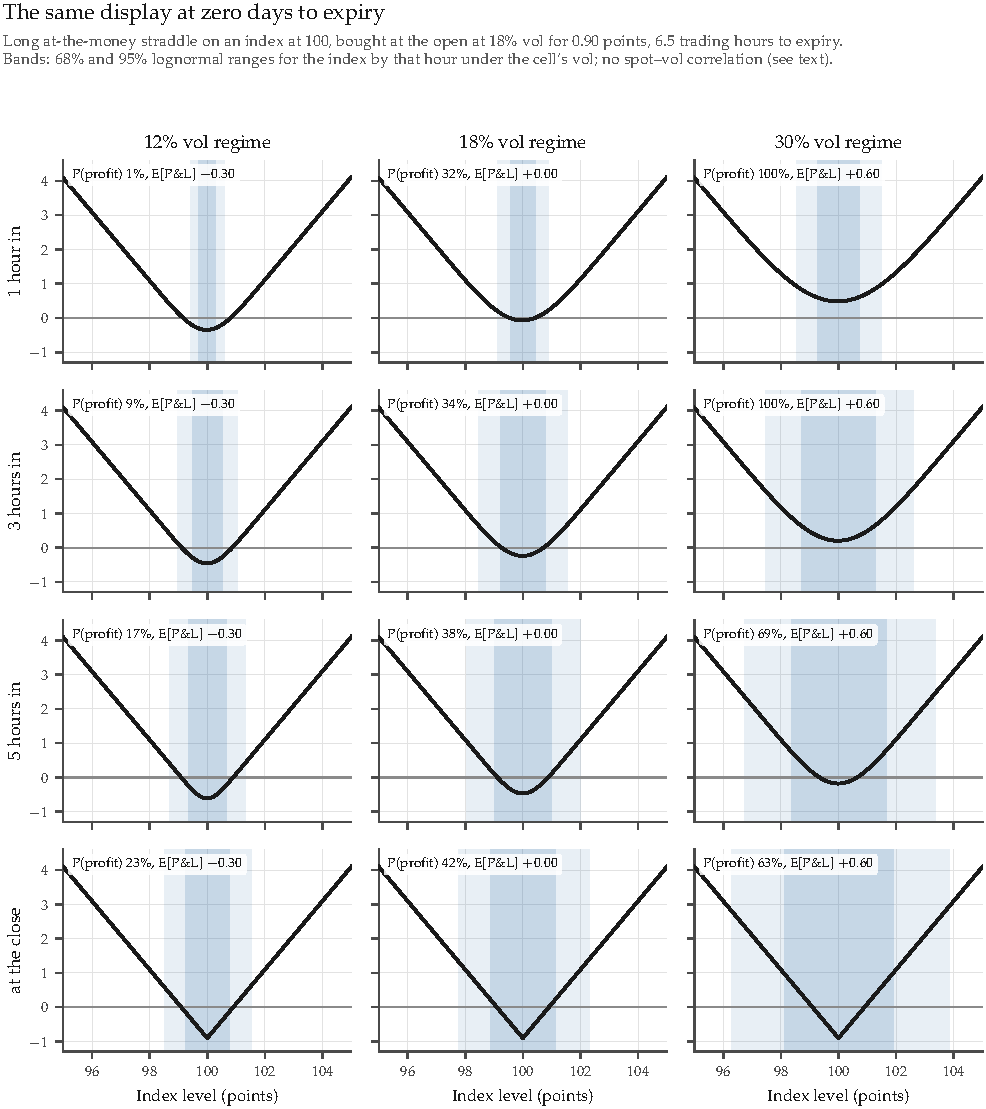
\includegraphics[width=0.92\linewidth]{v2_fig6.pdf}
\caption{The display at zero days to expiry: at-the-money straddle on an index at 100, bought at 18\% for 0.905 points, rows at one, three and five hours and at the close, columns at 12\%, 18\% and 30\% implied. Bands are unconditional lognormal ranges under each column's vol ($\rho = 0$; see text). Expected \PnL{} is constant down each column; the probability of profit is not. \emph{Status: illustrative scenario under a diffusion model that the text says does not transfer cleanly intraday; no calibration.}}
\end{figure}

\subsection{Against the Greeks, and three remarks}

A quant's first reaction is that the Greeks already say all this, and to a quant they do. Table~4 sets out the division of labour: a Greek is a local derivative, the grid a set of finite displacements under a measure, and the Greeks compose into a picture only in a head that can multiply a vega by a scenario whilst holding the theta, which describes the structurer and not the cohort de Silva, Smith and So measured. Three remarks. \emph{The drift:} bands are drawn under $\mu = r$ for consistency with the pricing model; for statements about likelihood the physical measure is the defensible choice and the user should supply $\mu$, but the display must not choose silently. \emph{The regimes:} flat repricings are a deliberate simplification; the natural extension prices cells off a smile-consistent shift under Heston or SABR dynamics, and the specification is agnostic to the engine. \emph{The frictions:} a grid that shows net-of-spread \PnL{} is the only version a regulator could sensibly mandate.

\begin{table}[htbp]
\centering\small
\caption{What the Greeks answer and what the grid answers.}
\begin{tabular}{@{}L{2.2cm}L{5.4cm}L{5.4cm}@{}}
\toprule
& The Greeks & The grid \\
\midrule
Nature & Local partial derivatives at $(S_0, 0, \sigma_0)$ & Finite displacements in $(S, u, \sigma)$ under a stated measure \\
Time & Theta: rate of decay now & Four dated curves; the convexity of decay visible \\
Volatility & Vega: sensitivity to a small move & Three regimes; the interaction with spot and time visible \\
Probability & None & Conditional bands, $P(\Pi>0)$, $E[\Pi]$, $Q_{5\%}(\Pi)$ per cell \\
Composition & In the reader's head & On the page \\
Audience & Those who already know what to look for & Those who demonstrably do not \\
\bottomrule
\end{tabular}
\end{table}

\section{Disclosure precedent: what PRIIPs got wrong}

\noindent An article arguing for a point-of-sale display standard owes an account of the last time one was tried. The EU's PRIIPs Key Information Document, from 2018, carried four performance scenarios computed from the product's own recent returns. The method was procyclical by construction: after a long bull market it produced scenarios that the FCA's own feedback statement of February 2019 recorded as ``misleading illustrations across almost all asset classes'' (FCA, 2019), and the regulator's remedy was to let providers attach explanatory material to a document whose purpose was to need none. The UK's response, in PS22/2 (FCA, 2022), was to remove the scenarios and require ``narrative information on performance'' instead, from 25 March 2022. A probabilistic display was mandated and then withdrawn because it lied.

The UK is now replacing PRIIPs wholesale: the Consumer Composite Investments framework (PS25/20; FCA, 2025) commences on 6 April 2026 with a transition to 8 June 2027, retains standardised content on costs, risk and return and past performance, and gives manufacturers ``considerable freedom over the design of product summaries''. For the avoidance of doubt, an exchange-traded option sold to a retail client will ordinarily fall within the CCI perimeter under DISC 1A.2.1R(1)(d), as a financial instrument which is a derivative, and none of the exclusions in DISC 1A.2.6R or regulation 4 of the Consumer Composite Investments Regulations 2024 captures it; which firm in the chain from exchange to broker owes the product summary is a separate question (FCA, 2026; SI 2024/1198). The regulator has moved from prescribing a probabilistic picture, to withdrawing it, to prescribing content and leaving design free: precisely the gap a display standard would fit, and precisely the gap the PRIIPs scenarios fell through. Three differences separate the proposal from the precedent: the PRIIPs measure came from the product's own past returns, the grid's from a stated model the user can change; the PRIIPs table hid its model, the grid prints its assumptions on its face; and the PRIIPs scenarios were never tested on readers before they were mandated.

\section{Implementation}

\noindent Table~5 is the specification a broker or risk platform would build from; the minimum column is modest work by the standards of what the platforms ship. Every rendering carries two disclosure lines, the status of each element (scenario, model-implied, historical, market-implied) and the spread assumption in force, and falls back to the static diagram with a notice when data are unavailable.

\begin{table}[htbp]
\centering\small
\caption{Implementation specification.}
\begin{tabular}{@{}L{2.4cm}L{5.0cm}L{5.6cm}@{}}
\toprule
Component & Minimum & Advanced \\
\midrule
Inputs & Position, spot, rate, one implied vol, three regime levels, $\sigma_R$, $\rho$, $\nu$, spread & Full surface, dividend and borrow curves, live bid--ask \\
Pricing & Black--Scholes & Smile-consistent stochastic-volatility model \\
Time grid & Fixed fractions of tenor & User-defined exit dates \\
Volatility & Three flat scenarios & Surface-consistent scenario shocks; vol-of-vol quantiles \\
Distribution & Conditional lognormal (Appendix~A) & Joint spot/volatility simulation with mean reversion and jumps \\
Outputs & $P(\Pi>0)$, $E[\Pi]$, $Q_{5\%}(\Pi)$, regime probability & Loss quantiles, expected shortfall, drawdown, margin path \\
Costs & User-specified proportional spread & Live bid--ask and slippage model \\
Refresh & At quote time; daily thereafter & Intraday, with the surface \\
Controls & Regime levels, $\sigma_R$, $\rho$, spread, mode & Custom measure and distribution upload \\
\bottomrule
\end{tabular}
\end{table}

\section{What would settle this}

\noindent The claim that the payoff diagram causes comprehension failures rests here on argument and proxy evidence, not on an experiment on readers. The experiment is cheap, and is specified so that it cannot be run loosely. \emph{Design:} between-subjects, five arms: i) the static payoff diagram; ii) the diagram plus a separate Greeks panel, to test whether any gain comes from the grid or merely from more information; iii) a slider tool matching broker practice, the important control; iv) the expert-mode grid; v) the retail-mode grid. Everything is preregistered. \emph{Participants:} retail investors who have traded a listed option, from a research panel; two attention checks (failure excludes), one manipulation check (reported). \emph{Tasks:} for the straddle of Section~2, estimate the \PnL{} of an unwind three weeks in under a stated vol change (primary); give the sign of the vega exposure; rank three outcomes by probability; locate the maximum loss; state the probability of profit at a date. Preference is asked last and analysed separately. \emph{Primary outcome and power:} absolute error on the primary task in units of the premium; a medium effect ($d = 0.5$) at $\alpha = 0.05$ and 80\% power needs 64 per arm for one contrast and 84 with Bonferroni over three primary contrasts, so 90 per arm, 450 in all. \emph{Practical significance:} mandate only if median absolute error halves relative to arm (i) or falls below 10\% of the premium. \emph{Hypotheses:} H1, arms (iv) and (v) beat (i) on the primary task; H2, they beat (iii) on the volatility and probability tasks; H3, (v) beats (iv) on the probability tasks; H4, arm (ii) does not close the gap to (iv). Falsifying H2 would mean the brokers have already solved the problem and Section~3 is wrong.

\section{Provenance, and a confession}

\noindent I first built this display in 2018, as an MSc project at City, University of London under Jason Dykes, in Excel and Tableau workarounds, each grid taking hours; the evaluation was a single-author use case, honestly weak, and the submitted version overlaid \emph{normal} bands on lognormal prices, an inconsistency I identified and ran out of runway to repair. The first rebuild for this article carried a second flaw: independent columns, and one volatility doing two jobs, so that a display designed to expose a suppressed parameter was silently overloading one. Section~4 is what it looks like when both are fixed. The rebuild took an evening, which is the second point of this piece: in 2018 the binding constraint was engineering effort; in 2026 it is nothing but the will of the platforms. The reproduction code for every figure and number is at github.com/phykit/payoff-diagram.

Until then, a display standard that shows retail users the geometry of $u = T$ under no measure at all, at the point of sale of same-day options, deserves to be called what it is. The payoff diagram tells you what happens \emph{if}. It has never once told you \emph{when}, \emph{how you get there}, or \emph{how likely}, and it is quite a lot to leave out.

\section*{Appendix A. Model, method and reproduction}

\noindent \emph{Notation and units.} $u$ is elapsed time since inception and $\tau = T - u$ the time remaining; the rows of Figure~4 are $u \in \{T/4, T/2, 3T/4, T\}$. Prices and \PnL{} are in unspecified units of currency: the 50 share is a hypothetical, and the two parameters taken from Apple, a correlation and a standard deviation of log changes, are dimensionless and independent of the currency in which Apple trades. All \PnL{} figures are per share, undiscounted, with the premium $V(S_0,T;\sigma_0)$ taken as paid in full at $u = 0$; one listed contract is 100 shares, so multiply by 100 for contract \PnL{}. Prices are mid-market unless a proportional spread $s$ is stated, in which case entry costs $V_0(1+s/2)$ and exit realises $V_u(1-s/2)$.

\emph{Pricing.} European Black--Scholes, continuous compounding, flat rate $r = 4\%$, no dividends, no borrow. Base case $S_0 = K = 50$, $\sigma_0 = 25\%$, $T = 0.5$ years; straddle premium $7.018$ (call $4.004$, put $3.014$). Figure~2 unwinds at $u = 21/250$; the minimum of the 45\% curve over spot is $+4.21$ at $S \approx 47.2$, against $+4.44$ at $S = 50$. In a general implementation, dividends enter as a continuous yield or discrete drops in $V$ and in the drift of $S_u$; a term structure of rates replaces $r$ by the zero rate to $\tau$; borrow cost enters as a negative yield; and the smile enters by pricing each cell off a surface shifted in a stated manner (parallel, sticky-strike or sticky-delta) rather than at a flat $\sigma_I$. None of these changes the display; each changes the numbers in it.

\emph{Vol regimes.} $\ln\sigma_u \sim N(\ln\sigma_0,\ \nu^2 u)$ with $\nu = 0.85$. Each column's $\sigma_I$ is a representative point value standing for a bucket, below 20\%, 20\% to 35\% and above 35\%; the regime probability printed in a cell is the probability of the bucket containing $\sigma_I$. The standardised vol move to the point value is $z = \ln(\sigma_I/\sigma_0)/(\nu\sqrt{u})$.

\emph{Conditional spot distribution.} With spot--vol correlation $\rho = -0.6$ and realised vol $\sigma_R$ over $[0,u]$, the joint law of $(\ln S_u, \ln\sigma_u)$ is taken to be bivariate normal, an assumption and not a derivation from a named stochastic-volatility model, and conditioning on the point value gives
\[
\ln S_u \,\big|\, \sigma_u = \sigma_I \;\sim\; N\!\Big(\ln S_0 + (\mu - \tfrac12\sigma_R^2)\,u + \rho\,\sigma_R\sqrt{u}\,z,\ \ (1-\rho^2)\,\sigma_R^2\,u\Big), \qquad \mu = r,
\]
with the default $\sigma_R = \sigma_I$. One convention needs stating because the probability and the shift are computed differently: the probability is that of the bucket, whilst the shift uses $z$ at the bucket's representative point. The alternative, shifting by the bucket-conditional mean $E[z \mid \text{bucket}]$ from the truncated normal, moves the 45\% column's conditional median from 41.2 to 42.5 at six weeks and from 40.2 to 38.7 at expiry; the point convention is used because the curve in the same cell is priced at the point, so curve and band describe the same state. The 68\% and 95\% bands are $\pm 1$ and $\pm 2$ conditional standard deviations about the conditional median. One consequence deserves a sentence: because conditioning on the regime removes the share of spot variance that vol movements explain, the middle column's expected \PnL{} is slightly negative even though its pricing vol is unchanged; a straddle in a world where vol demonstrably stayed put has, on average, seen less movement than it was priced for.

\emph{Cell statistics.} $P(\Pi > 0)$ and $E[\Pi]$ are computed by adaptive Gauss--Kronrod quadrature (SciPy \texttt{quad}, absolute tolerance $10^{-9}$) of $\Pi(S,u;\sigma_I)$ against the conditional density over $\pm 8$ conditional standard deviations in $\ln S$, with the indicator integral split at the median. $Q_{5\%}(\Pi)$ is the 5\% quantile of $\Pi$ on a 20,001-point probability-weighted grid over the same range. Convergence check: a 400,000-draw Monte Carlo under the same conditional law reproduces $P$, $E$ and $Q_{5\%}$ to within 0.002, 0.02 and 0.01 respectively in every cell tested (for example, three months in at 45\%: $1.000$, $+5.27$, $+1.82$ by quadrature against $1.000$, $+5.27$, $+1.82$ by simulation).

\emph{Calibration.} $\rho$ and $\nu$ are estimated from Apple, the only large single name with a free, official daily implied-volatility history: Cboe's VXAPL index (30-day implied volatility, published since 2011; Cboe, 2026b) against Apple's closing prices from Nasdaq (2026), 1 September 2021 to 3 September 2026, 1,257 matched trading days. Over non-overlapping horizons of one day, one week and one month the correlation of log spot changes with log implied-vol changes is $-0.60$, $-0.53$ and $-0.61$, and the annualised standard deviation of log implied-vol changes is $0.98$, $0.86$ and $0.83$; the one-month figures are used, since the display's rows are measured in months. Over the two years to September 2026 alone the corresponding monthly estimates are $-0.57$ and $0.91$. Two cautions. First, the quarterly-horizon vol-of-vol falls to $0.53$, because implied vol mean-reverts, so a lognormal vol process without mean reversion overstates dispersion at six months; the regime probabilities printed in the bottom row are model-implied and should be read as upper bounds on the tails. Over the five years Apple's implied vol was below 20\% on 4\% of days, between 20\% and 35\% on 80\%, and above 35\% on 15\%, against the model's 36\%, 36\% and 29\% at six months. A mean-reverting vol process is the natural refinement and changes nothing in the display specification. Second, the conditional shift is supported by few observations at the extreme: only three 21-day windows in five years saw implied vol rise by 80\% or more, and the share fell by 26\% on average in them.

\emph{Sensitivity to the vol law.} Replacing the lognormal vol law with a mean-reverting (Ornstein--Uhlenbeck) law in $\ln\sigma$, with reversion speed $\kappa = 6.9$ per year estimated from a monthly AR(1) on Apple's log implied vol (half-life about five weeks) and the same $\nu$, changes the two elements of the display in opposite directions (Table~6). The regime probabilities move towards the data: at six months, 16\%, 76\% and 7\% against the lognormal's 36\%, 36\% and 29\% and Apple's observed 4\%, 80\% and 15\%. The conditional shifts move away from it: with a tighter vol distribution the same 45\% regime is a larger standardised event, and the linear-Gaussian shift places the conditional median at 29.7 at expiry, a 41\% fall, where Apple's six-month windows ending in the high bucket show a fall of 19\% to 20\% relative to the middle bucket and the lognormal shift gives 20\%. The lognormal law is therefore kept for the shift, where it matches the data, and the appendix reports the mean-reverting probabilities as the better estimate of the column weights. The shift is the least robust element of the display and should be read as such.

\begin{table}[htbp]
\centering\small
\caption{Sensitivity of the bottom row (at expiry) to the vol law. Regime probability, probability of profit, expected \PnL{} and conditional median of spot, by column. Apple: six-month windows ending in each vol bucket, September 2021 to September 2026, spot return relative to the middle bucket.}
\begin{tabular}{@{}lrrrrrrrrr@{}}
\toprule
& \multicolumn{3}{c}{$P(\text{regime})$} & \multicolumn{3}{c}{$P(\Pi>0)$} & \multicolumn{3}{c}{Median spot} \\
\cmidrule(lr){2-4}\cmidrule(lr){5-7}\cmidrule(lr){8-10}
Vol law & 15\% & 25\% & 45\% & 15\% & 25\% & 45\% & 15\% & 25\% & 45\% \\
\midrule
Lognormal (display) & 36\% & 36\% & 29\% & 23\% & 32\% & 69\% & 53.5 & 50.2 & 40.2 \\
Mean-reverting, $\kappa = 6.9$ & 16\% & 76\% & 7\% & 62\% & 32\% & 93\% & 58.5 & 50.2 & 29.7 \\
Apple, observed & 4\% & 80\% & 15\% & & & & $+3\%$ & 0 & $-19\%$ \\
\bottomrule
\end{tabular}
\end{table}

\emph{Quantile dotplot.} Twenty dots at the conditional quantiles $(k - \tfrac12)/20$, $k = 1,\dots,20$, binned at width 2 along the price axis, coloured by the sign of $\Pi$ at the quantile.

\emph{0DTE grid.} Index at 100, $T = 1/252$ years for a 6.5-hour session, $\sigma_0 = 18\%$, premium $0.905$ points; columns 12\%, 18\%, 30\%; $\rho = 0$ and no regime probabilities, for the reason given in Section~4.

\emph{Frictions.} Round trip cost $= \tfrac{s}{2}\,V_0 + \tfrac{s}{2}\,V_u$ for a proportional spread $s$, with $V_0 = 7.018$ and $V_u = 11.46$ at unchanged spot; on Figure~2 the net curves are $V_u(S)(1-s/2) - V_0(1+s/2)$.

\emph{Reproduction.} All figures and every number quoted in the text are generated by two Python files (NumPy, SciPy, Matplotlib), the model in one and the figures in the other, typeset through pdfLaTeX so that figure text and body text share a face; a validation script prints the quoted numbers and the Monte Carlo check. The Apple and VXAPL series are archived with access dates. The package is at github.com/phykit/payoff-diagram (Kittson, 2026), with a one-command build.

\section*{References}
\begin{list}{}{\leftmargin=1.4em \itemindent=-1.4em \itemsep=4pt \topsep=6pt}
\item Bauer, R., Cosemans, M. and Eichholtz, P. (2009). Option trading and individual investor performance. \emph{Journal of Banking \& Finance}, 33(4), 731--746.
\item Bogousslavsky, V. and Muravyev, D. (2024). An anatomy of retail option trading. Working paper, SSRN 4682388.
\item Brown, A. (2022). Should individual investors trade options? \emph{Wilmott}, 2022. doi:10.54946/wilm.11024.
\item Charles Schwab (2026). \emph{Using options volatility data to research moves}. schwab.com/learn, accessed 4 September 2026.
\item Cboe Global Markets (2026a). \emph{State of the options industry: options market continued to break records in Q2 2026}. Cboe Insights, cboe.com, accessed 4 September 2026.
\item Cboe Global Markets (2026b). \emph{Cboe Equity VIX on Apple (VXAPL), daily history}. cdn.cboe.com/api/global/us\_indices/daily\_prices/VXAPL\_History.csv, accessed 4 September 2026.
\item Correll, M. and Gleicher, M. (2014). Error bars considered harmful: exploring alternate encodings for mean and error. \emph{IEEE Transactions on Visualization and Computer Graphics}, 20(12), 2142--2151.
\item de Silva, T., Smith, K. and So, E.C. (2026). Losing is optional: retail option trading and expected announcement volatility. \emph{Review of Finance}, 30(2), 489--535. doi:10.1093/rof/rfaf052.
\item E*TRADE (2026). \emph{Power E*TRADE options trading tools: Snapshot Analysis and TradeLab}. us.etrade.com/knowledge/library/options/trading-tools, accessed 4 September 2026.
\item Eaton, G.W., Green, T.C., Roseman, B.S. and Wu, Y. (2026). Retail option traders and the implied volatility surface. \emph{Journal of Financial Economics}, 177, 104238. doi:10.1016/j.jfineco.2026.104238.
\item Fei, T.T. and Prakash, E.C. (2001). Volume visualization of payoff regions for derivatives risk management. \emph{Journal of Visualization}, 4(4), 383--390.
\item Fernandes, M., Walls, L., Munson, S., Hullman, J. and Kay, M. (2018). Uncertainty displays using quantile dotplots or CDFs improve transit decision-making. \emph{Proceedings of the 2018 CHI Conference on Human Factors in Computing Systems}, paper 144.
\item Financial Conduct Authority (FCA) (2019). \emph{FS19/1: Call for Input on PRIIPs Regulation: initial experiences with the new requirements. Feedback statement}. February 2019.
\item Financial Conduct Authority (FCA) (2022). \emph{PS22/2: PRIIPs: final scope rules and amendments to Regulatory Technical Standards}. March 2022.
\item Financial Conduct Authority (FCA) (2026). \emph{FCA Handbook, DISC 1A: Consumer Composite Investments, General}, in force 6 April 2026. handbook.fca.org.uk/handbook/disc1a, accessed 4 September 2026.
\item Financial Conduct Authority (FCA) (2025). \emph{PS25/20: Supporting informed decision making: final rules for Consumer Composite Investments}. December 2025.
\item Gresh, D.L., Rogowitz, B.E., Tignor, M. and Mayland, E. (1999). An interactive framework for visualizing foreign currency exchange options. \emph{Proceedings of IEEE Visualization '99}, 453--456.
\item Hullman, J., Resnick, P. and Adar, E. (2015). Hypothetical outcome plots outperform error bars and violin plots for inferences about reliability of variable ordering. \emph{PLoS ONE}, 10(11), e0142444.
\item Interactive Brokers (2026a). \emph{Option Analytics}. interactivebrokers.co.uk/en/trading/option-analytics.php, accessed 4 September 2026.
\item Interactive Brokers (2026b). \emph{Probability Lab}. interactivebrokers.com/en/trading/probability-lab.php, accessed 4 September 2026.
\item Israelov, R. and Nielsen, L.N. (2014). Covered call strategies: one fact and eight myths. \emph{Financial Analysts Journal}, 70(6), 23--31.
\item Joslyn, S. and Savelli, S. (2021). Visualizing uncertainty for non-expert end users: the challenge of the deterministic construal error. \emph{Frontiers in Computer Science}, 2, 590232.
\item Kittson, S. (2026). \emph{payoff-diagram: reproduction package for ``The Payoff Diagram Is Lying to You''}. github.com/phykit/payoff-diagram, MIT licence, accessed 4 September 2026.
\item Ko, S., Cho, I., Afzal, S., Yau, C., Chae, J., Malik, A., Beck, K., Jang, Y., Ribarsky, W. and Ebert, D.S. (2016). A survey on visual analysis approaches for financial data. \emph{Computer Graphics Forum}, 35(3), 599--617.
\item Munzner, T. (2014). \emph{Visualization Analysis and Design}. AK Peters/CRC Press.
\item Nasdaq (2026). \emph{AAPL historical data}. nasdaq.com/market-activity/stocks/aapl/historical, accessed 4 September 2026; not redistributed.
\item OptionStrat (2026). \emph{Options profit calculator tutorial}. optionstrat.com/blog/options-profit-calculator-tutorial, accessed 4 September 2026.
\item OptionsProfitCalculator (2026). \emph{Frequently asked questions}. optionsprofitcalculator.com/faq.html, accessed 4 September 2026.
\item Padilla, L., Kay, M. and Hullman, J. (2022). Uncertainty visualization. In \emph{Wiley StatsRef: Statistics Reference Online}. Wiley.
\item The Consumer Composite Investments Regulations 2024, SI 2024/1198, regulation 4.
\item Tufte, E.R. (1983). \emph{The Visual Display of Quantitative Information}. Graphics Press.
\item Wystup, U. (2019). Shedding light on common misconceptions. \emph{Wilmott}, 2019(104). doi:10.1002/wilm.10801.
\end{list}

\vspace{8pt}
\noindent\rule{\linewidth}{0.4pt}\\[4pt]
{\small\itshape Simon Kittson is a solicitor (England \& Wales) and CFA charterholder specialising in derivatives and collateral. This article develops his 2018 MSc project at City, University of London, supervised by Jason Dykes. [Contact/bio line to author's preference.]}

\end{document}
